\section{Support Vector Machines}

\subsection{Hyperplanes and Margin Classification}

\begin{definition}{Support Vector Machine (SVM)}\\
    Goal: Find the optimal hyperplane that separates data points of different classes in a high-dimensional space. (maximize the margin between classes)\\
    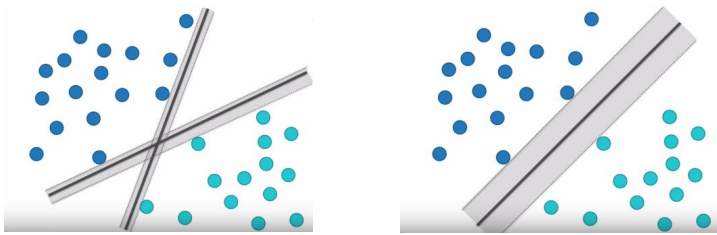
\includegraphics[width=\linewidth]{svms.png}
\end{definition}

\begin{definition}{Support Vector Machine (SVM)}\\
Support Vector Machines are supervised learning models used for classification and regression. In classification, SVMs find the hyperplane that best separates classes with the maximum margin.
\end{definition}

\begin{definition}{Hyperplane}\\
In $N$-dimensional space, a hyperplane is a flat affine subspace of dimensions $N-1$. In two dimensions, a hyperplane is a line defined by:
\[b + w_1 x_1 + w_2 x_2 = 0\]
In the general $N$-dimensional case:
\[b + w^T x = 0\]
\end{definition}

\begin{definition}{Support Vectors}\\
    Support vectors are the data points that are closest to the hyperplane and influence its position. They are critical for defining the optimal hyperplane.\\
    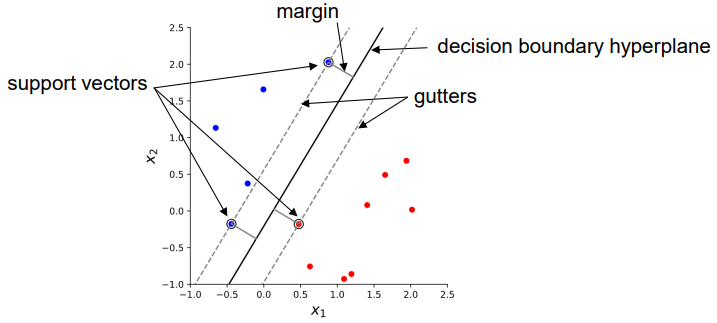
\includegraphics[width=\linewidth]{support_vectors.png}
\end{definition}

\begin{concept}{Optimisation Task for the Maximal Margin Classifier}\\
    The optimization task for the maximal margin classifier is to minimize the following objective function:
    \[ \min_{\mathbf{w}, b} \frac{1}{2} ||\mathbf{w}||^2 \quad \text{'Primal Form'}\]
    subject to the constraints:
    \[ y^{(m)} (b + \mathbf{w}^T \mathbf{x}^{(m)}) \geq 1, \quad \text{ for } m = 1,..., M \]
    where $\mathbf{w}$ is the weight vector, $b$ is the bias term, and $y^{(m)}$ is the class label of the $m$-th data point.
\end{concept}

\begin{definition}{Maximal Margin Classifier} Primal Form\\
    A maximal margin classifier finds the hyperplane that maximizes the distance to the nearest data point from any class. This leads to the optimization problem:
    \[\min_{b,w} \frac{1}{2}||w||^2\]
    subject to: $y^{(m)}(b + w^T x^{(m)}) \geq 1 \quad \forall m = 1,..., M$

    The data points closest to the hyperplane are called support vectors.
\end{definition}

\begin{concept}{Maximal Margin Classifier} Dual Form\\
The optimization problem for SVMs can be reformulated in its dual form:
\[\max_{\alpha} \mathcal{L}(\alpha) = - \frac{1}{2}\sum_{i=1}^{M}\sum_{j=1}^{M}\alpha_i\alpha_j y^{(i)}y^{(j)}x^{(i)}x^{(j)} + \sum_{m=1}^{M}\alpha_m\]
subject to: $\sum_{m=1}^{M}\alpha_m y^{(m)} = 0$ and $0 \leq \alpha_m \leq C$ for $m = 1, ..., M$

This formulation allows the application of the kernel trick by replacing the dot product $x^{(i)}x^{(j)}$ with a kernel function $\mathcal{K}(x^{(i)}, x^{(j)})$.
\end{concept}

\begin{theorem}{Predictions from the Optimised Lagrangian}\\
    With the optimal $\hat{\alpha}_m$ we can compute the optimal $\widehat{\mathbf{w}}$ from the equation in the previous slide
    \[ \widehat{\mathbf{w}}=\sum_{m=1}^M \hat{\alpha}_m y^{(m)} \mathbf{x}^{(m)} \]
    \[ \text{and }\hat{b}=\frac{1}{M_s} \sum_{m=1}^{M_s}\left(y^{(m)}-\widehat{\mathbf{w}}^T \mathbf{x}^{(m)}\right) \text{ for the support vectors}\]
    where $M_s$ is the number of support vectors and $\quad \hat{\alpha}_m>0$
    \vspace{2mm}\\
    Then, a new sample $\mathbf{x}^{(*)}$ can be classified using $y^{(*)}=\operatorname{sign}(\widehat{\mathbf{w}}^T \mathbf{x}^{(*)}+\hat{b})$
    The distance from the hyperplane can be interpreted as a confidence for the prediction.
\end{theorem}

\subsection{Kernel Trick and Soft Margin}

\begin{concept}{Hard Margin vs. Soft Margin}
\begin{itemize}
    \item \textbf{Hard Margin Classifier}: Requires all points to be correctly classified and outside the margin
    \item \textbf{Soft Margin Classifier}: Allows some points to violate the margin or be misclassified
\end{itemize}
The hard margin classifier works only when data is linearly separable and is sensitive to outliers.
\end{concept}

\begin{definition}{Soft Margin Classifier} Cost Function in Soft-Margin SVM\\
The soft margin classifier allows some data points to violate the margin constraints, adding \textbf{slack variables} $\varepsilon_m \geq 0$:
\[\min_{b,w,\varepsilon} \frac{1}{2}||w||^2 + C\sum_{m=1}^{M}\varepsilon^{(m)}\]
subject to: $y^{(m)}(b + \mathbf{w}^T \mathbf{x}^{(m)}) \geq 1 - \varepsilon^{(m)}$ and $\varepsilon^{(m)} \geq 0$ for $m = 1,..., M$

The parameter $C$ controls the trade-off between maximizing the margin and minimizing constraint violations.\\
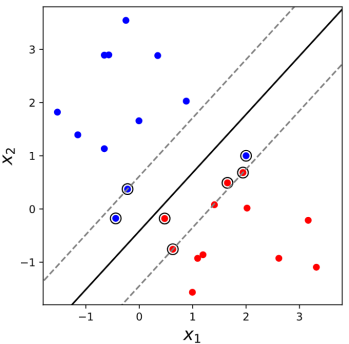
\includegraphics[width=0.5\linewidth]{softmargin_classifier.png}
\end{definition}

\begin{remark}
    Unbalanced data:\\
    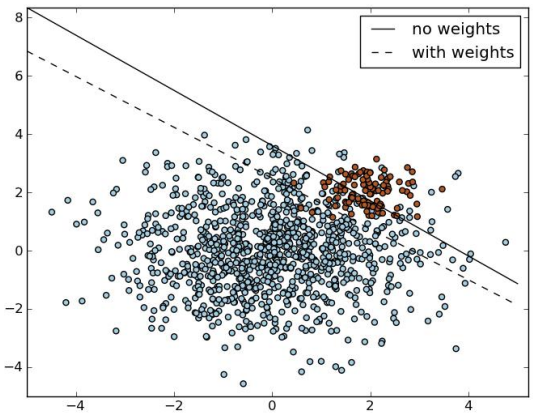
\includegraphics[width=0.5\linewidth]{unbalanced_data.png}
\end{remark}

\begin{example2}{'Wrong' Hyperplane}\\
    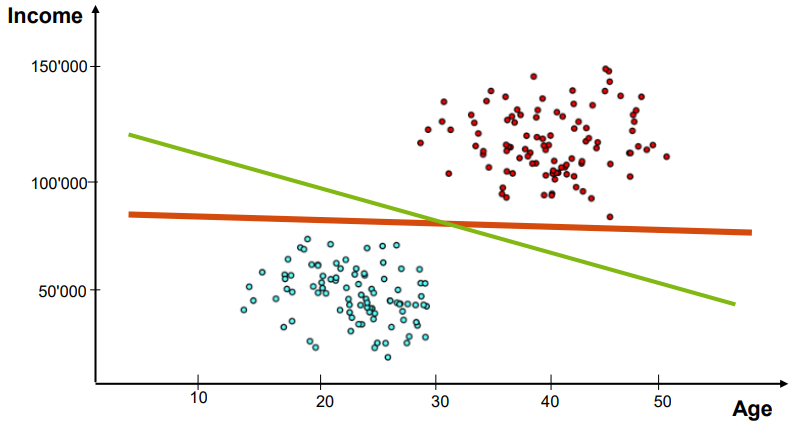
\includegraphics[width=\linewidth]{wrong_hyperplane.png}\\
    The \textcolor{red}{\textbf{RED}} line is the optimal hyperplane for the hard margin classifier. The \textcolor{green}{\textbf{GREEN}} line is NOT optimal!
\end{example2}

\begin{definition}{Standardization and Normalization}\\
    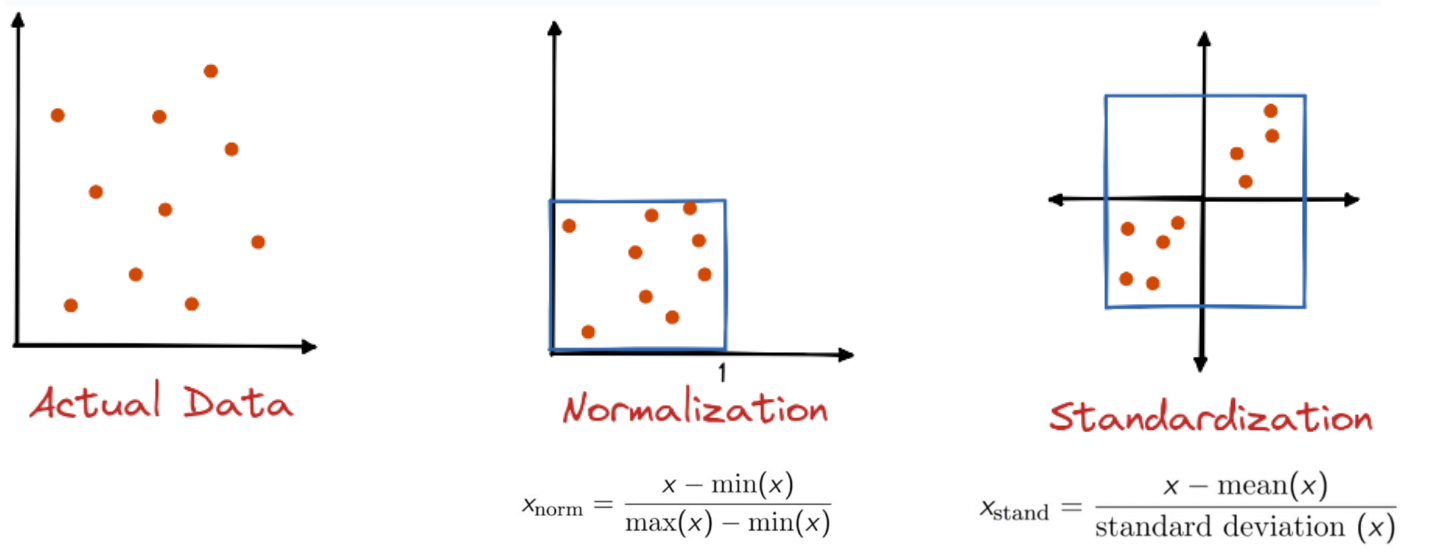
\includegraphics[width=\linewidth]{standardization_normalization.png}\\
    \small Normalization: e.g. for Neural Networks\\
    \small Standardization: e.g. for SVMs, Linear and Logistic Regression    
\end{definition}

\subsubsection{Kernel Trick for non-linearly seperable data}

\begin{definition}{Lifting Trick} Projection to Higher Dimensions\\
    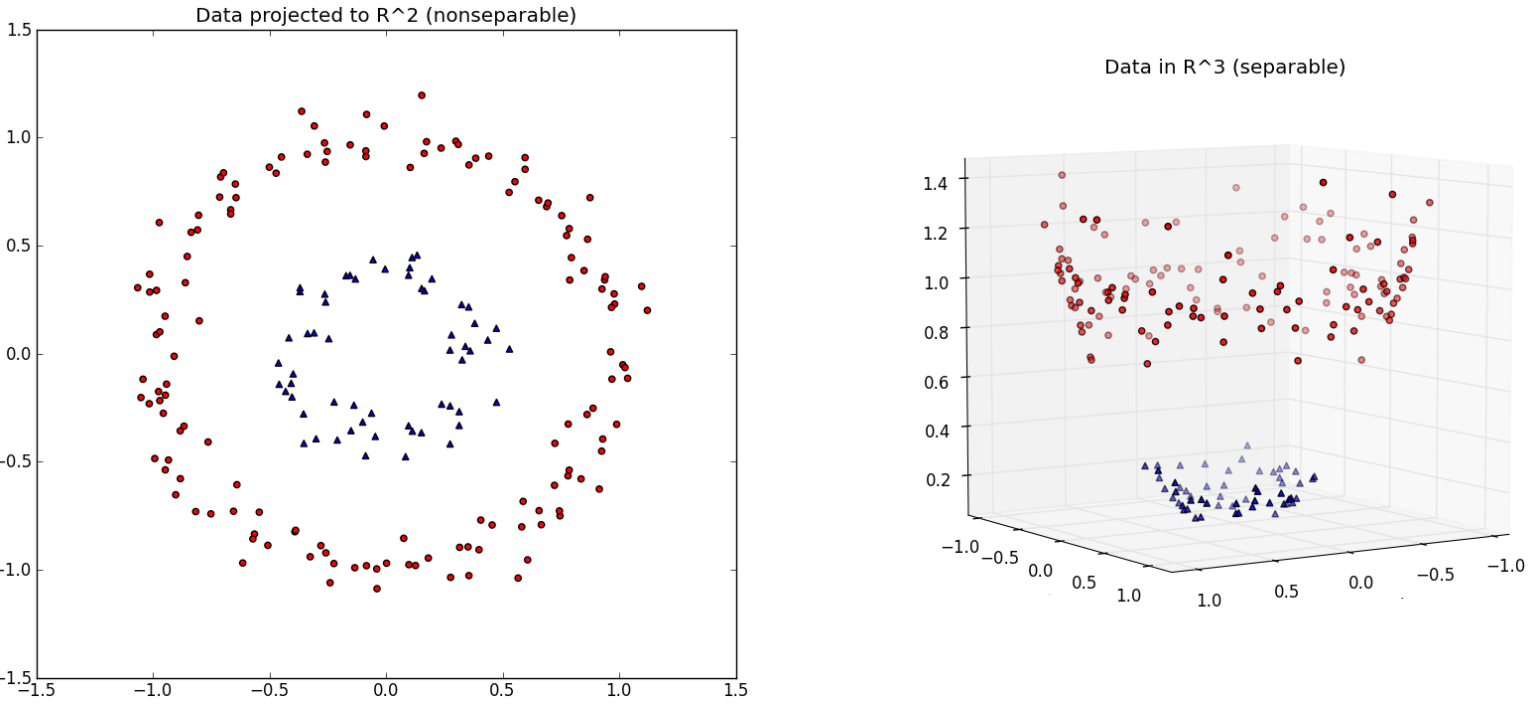
\includegraphics[width=\linewidth]{lifting_trick.png}\\
    Transformation: $(x_1, x_2) \rightarrow (x_1, x_2, x_1^2 + x_2^2)$\\
    \small The lifting trick allows us to transform the data into a higher-dimensional space where it may become linearly separable.
\end{definition}

\begin{concept}{Kernel Trick}\\
The kernel trick allows SVMs to efficiently operate in high-dimensional spaces without explicitly computing the transformation. Common kernels include:
\begin{itemize}
    \item Linear: $\mathcal{K}(x^{(m)}, x^{(m')}) = \sum_{n=1}^{N} x^{(m)}_n x^{(m')}_n$
    \item Polynomial: $\mathcal{K}(x^{(m)}, x^{(m')}) = (1 + \sum_{n=1}^{N} x^{(m)}_n x^{(m')}_n)^d$
    \item RBF: $\mathcal{K}(x^{(m)}, x^{(m')}) = \exp(-\gamma||x^{(m)} - x^{(m')}||^2)$
\end{itemize}
\end{concept}

\begin{theorem}{Maximal Margin Classifier} Dual Form with Kernel Trick
\[\max_{\alpha} \mathcal{L}(\alpha) = - \frac{1}{2}\sum_{i=1}^{M}\sum_{j=1}^{M}\alpha_i\alpha_j y^{(i)}y^{(j)} \textcolor{pink}{\mathcal{K}(x^{(i)}, x^{(j)})} + \sum_{m=1}^{M}\alpha_m\]
subject to: $\sum_{m=1}^{M}\alpha_m y^{(m)} = 0$ and $0 \leq \alpha_m \leq C$ for $m = 1, ..., M$

This formulation allows the application of the kernel trick by replacing the dot product $x^{(i)}x^{(j)}$ with a kernel function $\mathcal{K}(x^{(i)}, x^{(j)})$.
\end{theorem}

\begin{formula}{Common Kernel Functions}

    \begin{minipage}{0.7\linewidth}
    Linear: $\quad K(a, b)=a^{\top} \cdot b$

    Polynomial: $\quad K(a, b)=\left(a^{\top} \cdot b+t\right)^r$ with parameters $\mathbf{t}, \mathbf{r}$

    RBF = Radial Basis Function:
    \[ \mathrm{K}(\mathrm{a}, \mathrm{~b})=e^{-\gamma\|a-b\|^2} \]
    with parameter $\gamma$
    \end{minipage}
    \begin{minipage}{0.25\linewidth}
        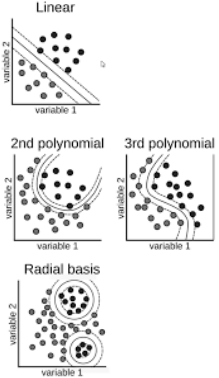
\includegraphics[width=\linewidth]{common_kernel_functions.png}
    \end{minipage}
\end{formula}



\begin{KR}{Selecting the Right Kernel and Parameters}
\paragraph{When to use different kernels}
\begin{itemize}
    \item Linear kernel: 
    \begin{itemize}
        \item When data is linearly separable
        \item When feature space is large compared to sample size
        \item For text classification problems
    \end{itemize}
    \item Polynomial kernel:
    \begin{itemize}
        \item When decision boundary is a curved line or surface
        \item For image processing problems
        \item Typical degrees: 2 or 3
    \end{itemize}
    \item RBF kernel:
    \begin{itemize}
        \item When classes form complex shapes
        \item For most general-purpose classification
        \item When you have sufficient data
    \end{itemize}
\end{itemize}

\paragraph{Parameter tuning}
\begin{itemize}
    \item Use grid search or random search with cross-validation
    \item C parameter search range: $[0.1, 1, 10, 100, 1000]$
    \item For RBF kernel, $\gamma$ search range: $[0.01, 0.1, 1, 10]$
    \item For polynomial kernel, degree values: $[2, 3, 4]$
\end{itemize}

\paragraph{Optimize for the metric that matters}
\begin{itemize}
    \item Accuracy for balanced problems
    \item F1-score for imbalanced problems
    \item Precision or recall when false positives or false negatives are more critical
\end{itemize}
\end{KR}

\begin{definition}{RBF Kernel}
    \[ \mathrm{K}(\mathrm{a}, \mathrm{~b}) = e^{-\gamma\|a-b\|^2} = e^{-\frac{||a-b||^2}{2\sigma^2}} \]
    Small $\gamma \rightarrow$ large width $\sigma$ (Gaussian kernel)\\
    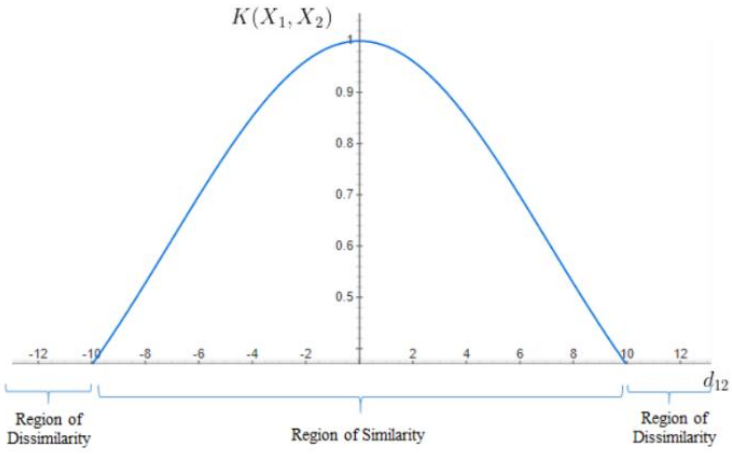
\includegraphics[width=\linewidth]{small_gamma.png}\\
    Large $\gamma \rightarrow$ small width $\sigma$ (Gaussian kernel)\\
    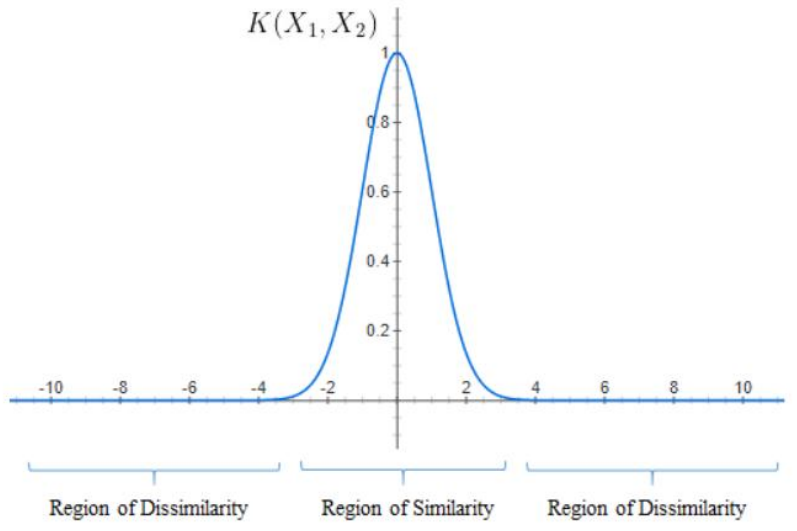
\includegraphics[width=\linewidth]{large_gamma.png}
\end{definition}

\begin{example2}{RBF Kernel}\\
    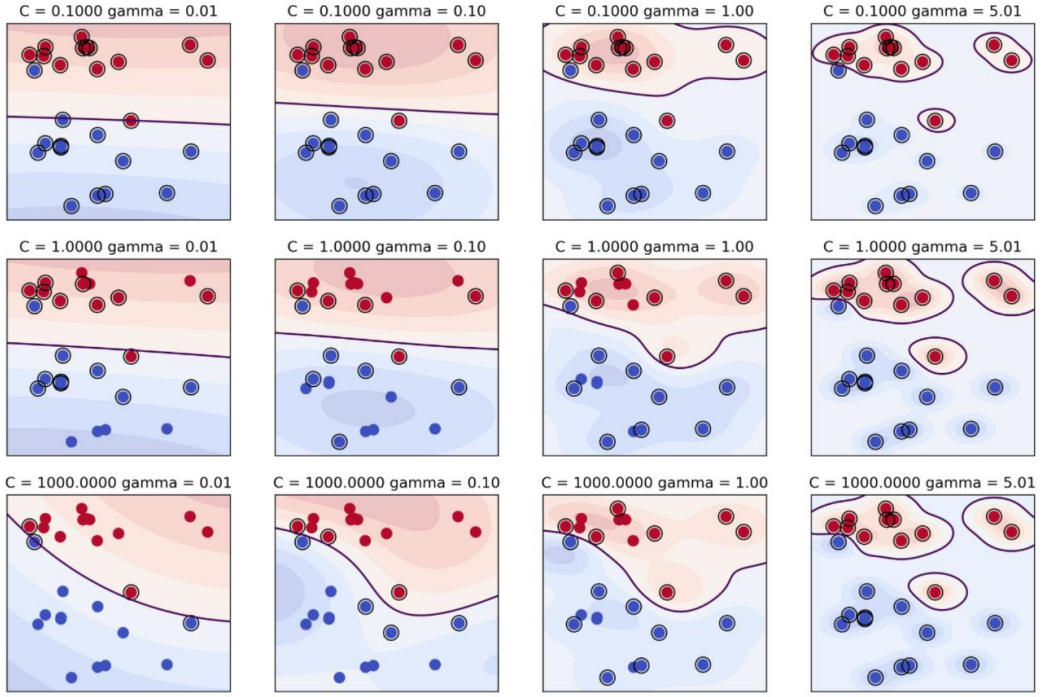
\includegraphics[width=\linewidth]{rbfkernel.png}
\end{example2}

\begin{theorem}{Interdependence of SVM Hyperparameters}\\
    $C$ and $\gamma$ both influence the shape of the decision boundary and need to be tuned together 
    using hyperparameter optimization (e.g. via cross validation)
\end{theorem}

\begin{example2}{ConceptTest: RBF Kernel}\\
    In the SVM below we are using $\mathrm{C}=1$. Which image has the highest value for hyperparameter $\gamma$ ?

    \[ K\left(\mathbf{x}, \mathbf{x}^{(m)}\right)=\exp \left(-\gamma\left\|\mathbf{x}^{(m)}-\mathbf{x}\right\|^2\right) \]

    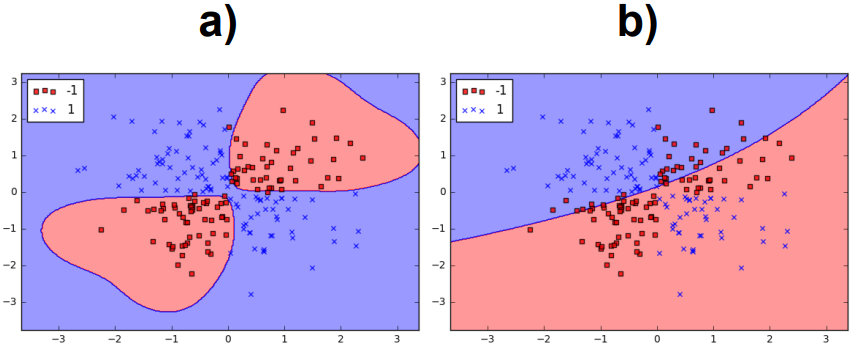
\includegraphics[width=\linewidth]{rbfexample1.png}\\
    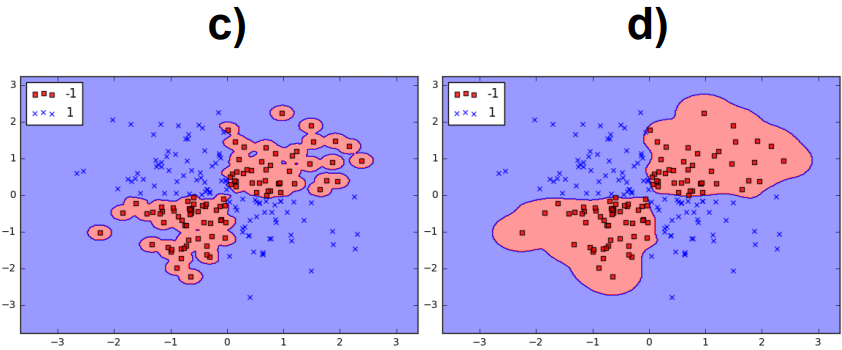
\includegraphics[width=\linewidth]{rbfexample2.png}
\end{example2}

\begin{example}{SVM Application} Linear Kernel\\
Consider classifying flowers based on petal length and width:
\begin{itemize}
    \item Features: Petal length ($x_1$) and petal width ($x_2$)
    \item Classes: Setosa (-1) and Versicolor (+1)
    \item After training with a linear kernel, we get $b = -0.5$ and $w = [0.2, 0.8]$
    \item For a new flower with petal length = 4 cm and width = 1.3 cm:
    \begin{itemize}
        \item $f(x) = -0.5 + 0.2 \times 4 + 0.8 \times 1.3 = -0.5 + 0.8 + 1.04 = 1.34 > 0$
        \item Prediction: Versicolor (class +1)
    \end{itemize}
\end{itemize}
\end{example}

\begin{KR}{Training a Support Vector Machine}
    \paragraph{Select kernel}
    Choose an appropriate kernel function:
    \begin{itemize}
        \item Linear kernel for linearly separable data
        \item Polynomial kernel for more complex, non-linear boundaries
        \item RBF (Gaussian) kernel for highly non-linear data
    \end{itemize}
    
    \paragraph{Select hyperparameters}
    \begin{itemize}
        \item $C$: Regularization parameter (controls trade-off between margin width and misclassification)
        \item Kernel parameters: degree $d$ for polynomial kernel, $\gamma$ for RBF kernel
    \end{itemize}
    
    \paragraph{Train the model}
    \begin{itemize}
        \item Set up the optimization problem to maximize the margin
        \item Solve the quadratic programming problem to find support vectors
    \end{itemize}
    
    \paragraph{Make predictions}
    For a new data point $x$:
    \begin{itemize}
        \item Compute $f(x) = b + \sum_{i \in SV} \alpha_i y_i K(x_i, x)$
        \item Predict class 1 if $f(x) > 0$, otherwise class -1
    \end{itemize}
    \end{KR}

\subsection{Multi-class Classification with SVMs}

\begin{concept}{Multi-class SVM}\\
SVMs are inherently binary classifiers. For multi-class problems, approaches include:
\begin{itemize}
    \item \textbf{One-vs-All}: Train $K$ SVMs, each separating one class from all others
    \item \textbf{One-vs-One}: Train $\binom{K}{2}$ SVMs, each separating one class from another
\end{itemize}
\end{concept}

\begin{definition}{One-vs-All (One-vs-Rest) Approach}\\
In the one-vs-all approach:
\begin{itemize}
    \item Train $K$ binary classifiers, one for each class
    \item For each classifier, positive examples are from one class, negative examples from all other classes
    \item For prediction, apply all classifiers and select the class with highest confidence (furthest from the decision boundary)
\end{itemize}
\end{definition}

\begin{definition}{One-vs-One Approach}\\
In the one-vs-one approach:
\begin{itemize}
    \item Train $\binom{K}{2} = \frac{K(K-1)}{2}$ binary classifiers, one for each pair of classes
    \item For prediction, each classifier votes for one class
    \item The class with the most votes wins
\end{itemize}
\end{definition}

\begin{example2}{Multi-class Classification}\\
Consider a flower classification problem with three classes: Setosa, Versicolor, and Virginica.
\begin{itemize}
    \item Features: Petal length and petal width
    \item One-vs-All approach:
    \begin{itemize}
        \item Classifier 1: Setosa vs. non-Setosa
        \item Classifier 2: Versicolor vs. non-Versicolor
        \item Classifier 3: Virginica vs. non-Virginica
    \end{itemize}
    \item One-vs-One approach:
    \begin{itemize}
        \item Classifier 1: Setosa vs. Versicolor
        \item Classifier 2: Setosa vs. Virginica
        \item Classifier 3: Versicolor vs. Virginica
    \end{itemize}
\end{itemize}
\tcblower
For a new flower with petal length = 5 cm and width = 1.8 cm:

One-vs-All approach:
\begin{itemize}
    \item Classifier 1 (Setosa vs. rest): $f_1(x) = -3.5 < 0$ (not Setosa)
    \item Classifier 2 (Versicolor vs. rest): $f_2(x) = -0.8 < 0$ (not Versicolor)
    \item Classifier 3 (Virginica vs. rest): $f_3(x) = 2.3 > 0$ (Virginica)
\end{itemize}
Prediction: Virginica

One-vs-One approach:
\begin{itemize}
    \item Classifier 1 (Setosa vs. Versicolor): Votes for Versicolor
    \item Classifier 2 (Setosa vs. Virginica): Votes for Virginica
    \item Classifier 3 (Versicolor vs. Virginica): Votes for Virginica
\end{itemize}
Virginica gets 2 votes, Versicolor gets 1 vote, Setosa gets 0 votes.
Prediction: Virginica
\end{example2}

\subsection{SVM for Regression}

\begin{definition}{Support Vector Regression (SVR)}\\
SVR applies the same principles as SVM to regression tasks by:
\begin{itemize}
    \item Fitting as many instances as possible on a "street" with width controlled by parameter $\varepsilon$
    \item Allowing some points to be off the street (margin violations)
    \item Using kernels to handle non-linear regression tasks
\end{itemize}
\end{definition}

\begin{concept}{Key Differences Between SVR and Linear Regression}
\begin{itemize}
    \item Linear regression minimizes the squared error for all points
    \item SVR is only concerned with errors larger than $\varepsilon$ (the tube width)
    \item SVR is more robust to outliers
    \item SVR produces a sparse solution (depends only on support vectors)
\end{itemize}
\end{concept}

\begin{KR}{Implementing Support Vector Regression}
\paragraph{Define the problem}
\begin{itemize}
    \item Determine if a non-linear relationship exists in the data
    \item Decide if robustness to outliers is important
\end{itemize}

\paragraph{Select parameters}
\begin{itemize}
    \item $\varepsilon$: Controls the width of the insensitive tube (larger $\varepsilon$ means fewer support vectors)
    \item $C$: Regularization parameter (smaller $C$ means more regularization)
    \item Kernel and its parameters (same as for SVM classification)
\end{itemize}

\paragraph{Train and evaluate}
\begin{itemize}
    \item Train using appropriate solver
    \item Evaluate using metrics like MSE, MAE, or $R^2$
    \item Tune parameters using cross-validation
\end{itemize}
\end{KR}

\begin{example}{SVR Example}
Consider predicting house prices based on size (in square feet):
\begin{itemize}
    \item Training data: 100 houses with sizes ranging from 1000 to 3000 sq ft and prices from \$200,000 to \$600,000
    \item We use SVR with an RBF kernel, $C=1000$, $\varepsilon=10000$, and $\gamma=0.0001$
    \item For a new house with 2500 sq ft:
    \begin{itemize}
        \item Predicted price: \$475,000
        \item Only 15 support vectors were used for this prediction (out of 100 training examples)
    \end{itemize}
\end{itemize}
\end{example}